%=========================================================
\chapter{Modelo de manejo de la información.}	

El modelo de manejo de la información es un aspecto crucial en el diseño del sistema de la guardería "Guardería Burbujas". Este modelo se enfoca en cómo se gestiona y accede a la información dentro del sistema, especialmente a través de consultas a la base de datos. El manejo efectivo de la información es fundamental para garantizar un funcionamiento óptimo del sistema y satisfacer las necesidades de los usuarios.

En el contexto de la guardería "Guardería Burbujas", el modelo de manejo de la información se centra en cómo se almacenan y recuperan los datos relacionados con los niños, los padres, las actividades, los horarios y otros aspectos relevantes para la gestión de la guardería. Una base de datos es utilizada para almacenar esta información de manera estructurada y eficiente.
\\

El modelo de manejo de la información se basa en el uso de consultas para acceder y manipular los datos almacenados en la base de datos. Las consultas son instrucciones o comandos que se envían a la base de datos para recuperar información específica de acuerdo a ciertos criterios o realizar operaciones de actualización en los datos.

En el sistema de la guardería "Guardería Burbujas", se utilizan consultas para diversas funcionalidades, como:

\begin{itemize}
\item Obtener la lista de niños y sus datos personales.
\item Buscar los horarios de las actividades para un día determinado.
\item Registrar la asistencia de los niños a las actividades.
\end{itemize}

Para realizar estas consultas, se utilizan lenguajes de consultas se usan funciones de \textbf{Mongoose} para la base de datos MongoDB que pueden ser usadas tambien en \textbf{CosmosDB}

El diseño adecuado del modelo de manejo de la información es esencial para garantizar un acceso eficiente y preciso a los datos en el sistema de la guardería "Guardería Burbujas". Se deben considerar aspectos como la estructura de la base de datos, la indexación de los datos, la optimización de consultas y la seguridad de la información.
\\

En este capítulo, se presentarán las técnicas y consideraciones clave en el diseño del modelo de manejo de la información en el sistema de la guardería "Guardería Burbujas". Se analizará la estructura de la base de datos que son collecciones en base a las entidades previamente echas.


\begin{figure}[htbp]
\centering
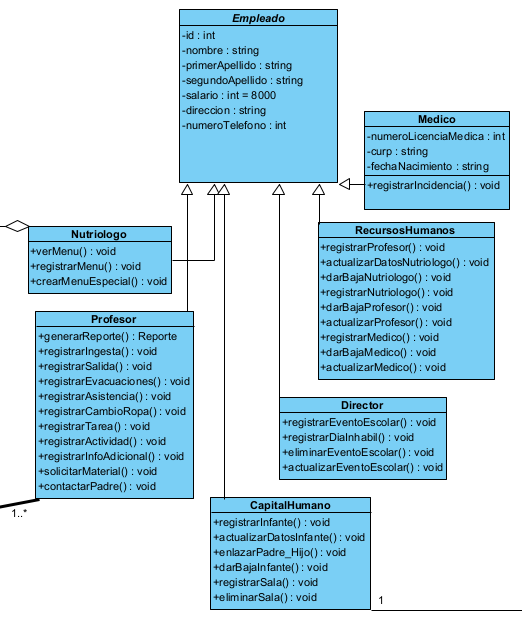
\includegraphics[width=0.4\textwidth]{images/arqui/comEmpleados.png}
\caption{Diagrama de la coleccion de las entidades de los empleados}
\label{fig:colecEmp}
\end{figure}

\begin{figure}[htbp]
\centering
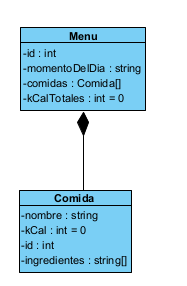
\includegraphics[width=0.4\textwidth]{images/arqui/colmenuComida.png}
\caption{Diagrama de la coleccion del menu y las comidas}
\label{fig:colecMenucCOM}
\end{figure}

\begin{figure}[htbp]
\centering
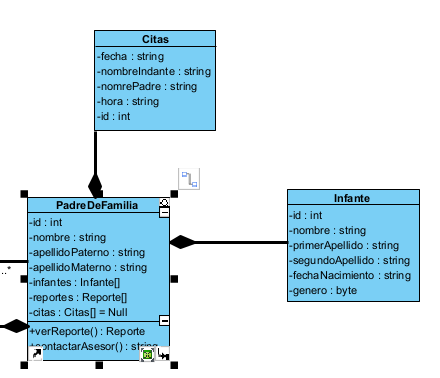
\includegraphics[width=0.4\textwidth]{images/arqui/colPadreFamilia.png}
\caption{Diagrama de la coleccion deL padre de familia}
\label{fig:colecPadre}
\end{figure}

\begin{figure}[htbp]
\centering
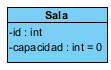
\includegraphics[width=0.4\textwidth]{images/arqui/sala.png}
\caption{Diagrama de la coleccion de una sala}
\label{fig:colecSala}
\end{figure}

\begin{figure}[htbp]
\centering
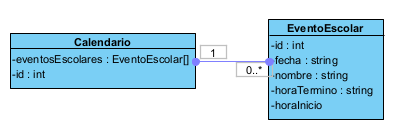
\includegraphics[width=0.4\textwidth]{images/arqui/colCaEv.png}
\caption{Diagrama de la coleccion deL calendario con Eventos Escolares}
\label{fig:colecEventCald}
\end{figure}
\clearpage

%======================================================================
\section{Consultas para el Caso de Uso CU1}

\begin{itemize}
    \item \textbf{Consulta001} usada para registrar un profesor
\end{itemize}

\begin{verbatim}
const nuevoProfesor = new Profesor({
  nombre: <nombreProfesor>,
  direccion: <direccionProfesor>,
  numeroTelefono: <numeroTelefonoProfesor>
});
    
nuevoProfesor.save();
\end{verbatim}


%======================================================================
\section{Consultas para el Caso de Uso CU2}

\begin{itemize}
    \item \textbf{Consulta002} usada para registrar un padre de familia.
\end{itemize}

\begin{verbatim}
const nuevoPadre = new PadredeFamilia({
  nombre: <nombrePadre>,
  direccion: <direccionPadre>,
  numeroTelefono: <numeroTelefonoPadre>
});
    
nuevoPadre.save();
\end{verbatim}


%======================================================================
\section{Consultas para el Caso de Uso CU3}

\begin{itemize}
    \item \textbf{Consulta003} usada para registrar un infante en el sistema.
\end{itemize}

\begin{verbatim}
const nuevoInfante = new Infante({
  nombre: <nombreInfante>,
  direccion: <direccionInfante>,
  fechaNacimiento: <fechaNacimientoInfante>
});
    
nuevoPadre.save();
\end{verbatim}


%======================================================================
\section{Consultas para el Caso de Uso CU4}

\begin{itemize}
    \item \textbf{Consulta004} usada para enlazar un padre con su hijo en la guarderia
\end{itemize}

\begin{verbatim}
Padre.findOne({ id: <idPadre> }).exec((error, padre) => {
  if (error) {
    console.log(error);
  } else {
    padre.infantes.push(<infante>);
    padre.save();
  }
});
\end{verbatim}


%======================================================================
\section{Consultas para el Caso de Uso CU5}

\begin{itemize}
    \item \textbf{Consulta005} llenado de datos de una sala para ser registrada
\end{itemize}

\begin{verbatim}
const nuevaSala = new Sala({
  capacidad: <numeroCapacidad>,
});
    
nuevaSala.save();
\end{verbatim}


%======================================================================
\section{Consultas para el Caso de Uso CU6}

\begin{itemize}
    \item \textbf{Consulta006} registro de un nuevo nutriologo
\end{itemize}

\begin{verbatim}
const nuevoNutriologo = new Nutriologo({
  nombre: <nombreNutriologo>,
  direccion: <direccionNutriologo>,
  numeroTelefono: <numeroTelefonoNutriologo>
});
    
nuevoNutriologo.save();

\end{verbatim}

\begin{itemize}
    \item \textbf{Consulta026} Eliminar nutriologo
\end{itemize}

\begin{verbatim}


nutriologo = Nutriologo.findOne({nombre: <nombreNutriologo> });

Nutriologo.deleteOne({id: <nutriolog.id> });
\end{verbatim}


%======================================================================
\section{Consultas para el Caso de Uso CU7}

\begin{itemize}
    \item \textbf{Consulta007} registro de comidas para el menu
\end{itemize}

\begin{verbatim}
const nuevoMenu = new Menu({
  momentoDelDia: <momentoDelDiaMenu>,

});
nuevoMenu.save();


const nuevaComida = new Comida({
  nombre: <nombreComida>,
  kCal: <numeroKCalorias>,
  ingredientes: <ingredientesComida>
});
    
nuevaComida.save();
nuevoMenu.comidas.push(nuevaComida);
nuevoMenu.save();

\end{verbatim}


%======================================================================
\section{Consultas para el Caso de Uso CU8}

\begin{itemize}
    \item \textbf{Consulta008} generar Cita con tutor
\end{itemize}

\begin{verbatim}
const nuevaCita = new Cita({
  nomreInfante: <nombreInfante>,
  nomrePadre: <nombrePadre>,
  fecha: <fechaCita>,
  hora: <horaCita>,
});
nuevaCita.save();

padre.citas.push(nuevaCita);
padre.save();

\end{verbatim}

%======================================================================
\section{Consultas para el Caso de Uso CU9}

\begin{itemize}
    \item \textbf{Consulta009} registrar ingesta en el reporte
\end{itemize}

\begin{verbatim}
reporteInfanteA.ingesta.push(<Ingesta>);
reporteInfanteA.save();
\end{verbatim}


%======================================================================
\section{Consultas para el Caso de Uso CU11}

\begin{itemize}
    \item \textbf{Consulta011} registrar actividades realizadas en el reporte
\end{itemize}

\begin{verbatim}
reporteInfanteA.actividades.push(<ActividadRealizada>);
reporteInfanteA.save();
\end{verbatim}

%======================================================================
\section{Consultas para el Caso de Uso CU12}

\begin{itemize}
    \item \textbf{Consulta012} registrar tareas en el reporte
\end{itemize}

\begin{verbatim}
reporteInfanteA.tareas.push(<tarea>);
reporteInfanteA.save();
\end{verbatim}

%======================================================================
\section{Consultas para el Caso de Uso CU14}

\begin{itemize}
    \item \textbf{Consulta014} registra medico en el sistema
\end{itemize}

\begin{verbatim}

const nuevoMedico = new Medico({
  nombre: <nombreMedico>,
  direccion: <direccionMedico>,
  numeroTelefono: <numeroTelefonoMedico>,
  numeroLicenciaMedica: <numeroLicenciaMedico>,
  curp: <curpMedico>,
  fechaNacimiento: <fechaNacimientoMedico>
});
    
nuevoMedico.save();

\end{verbatim}



\begin{itemize}
    \item \textbf{Consulta025} eliminar medico en el sistema
\end{itemize}

\begin{verbatim}
medico = Medico.findOne({nombre: <nombreMedico> });

Medico.deleteOne({id: <medico.id> });



\end{verbatim}

%======================================================================
\section{Consultas para el Caso de Uso CU15}

\begin{itemize}
    \item \textbf{Consulta015} registrar incidencia medica en el reporte
\end{itemize}

\begin{verbatim}
incidencia = ["Incidencia medica:", <Detalles>, <Estado infante>]
reporteInfanteA.informacionAdicional.push(<incidencia>);
\end{verbatim}

%======================================================================
\section{Consultas para el Caso de Uso CU17}

\begin{itemize}
    \item \textbf{Consulta017} registrar evento escolar
\end{itemize}

\begin{verbatim}
const nuevoEvento = new Evento({
  nombre: <nombreEvento>,
  fecha: <fechaEvento>,
  horaInicio: <horaInicioEvento>,
  horaTermino: <horaTerminoEvento>
});
nuevoEvento.save();
calendario.eventosEscolares.push(nuevoEvento);
calendario.save();
\end{verbatim}

\begin{itemize}
    \item \textbf{Consulta024} Eliminar evento escolar
\end{itemize}

\begin{verbatim}
calendario.updateOne(
  { $pull: { eventosEscolares: { id: <nuevoEvento.id> } } } 
);
\end{verbatim}


%======================================================================
\section{Consultas para el Caso de Uso CU19}

\begin{itemize}
    \item \textbf{Consulta019} Para que el profesor registre asistencia de los infantes
\end{itemize}

\begin{verbatim}
reporteInfanteA.asistencia = True;
reporteInfanteA.save();
\end{verbatim}

%======================================================================
\section{Consultas para el Caso de Uso CU22}

\begin{itemize}
    \item \textbf{Consulta022} El profesor registra el reporte del infante
\end{itemize}

\begin{verbatim}
const nuevoReporte = new Reporte({
  asistencia: <asistenciaInfante>,
  evacuaciones: <evacuacionesInfate>,
  ingesta: <ingestaInfante>,
  cambioRopa: <cambioRopaInfante>,
  actividades: <actividadesInfante>,
  tareas: <tareasInfante>,
  fecha: Date.now
});
nuevoReporte.save();

padre.reportes.push(nuevoReporte)
\end{verbatim}
